\documentclass[
11pt, % The default document font size, options: 10pt, 11pt, 12pt
codirector, % Uncomment to add a codirector to the title page
]{charter} 

\usepackage{svg}
\usepackage{tabularx}


% El títulos de la memoria, se usa en la carátula y se puede usar el cualquier lugar del documento con el comando \ttitle
\titulo{Inteligencia Artificial en sistemas embebidos} 

% Nombre del posgrado, se usa en la carátula y se puede usar el cualquier lugar del documento con el comando \degreename
\posgrado{Carrera de Especialización en Inteligencia Artificial}

% Tu nombre, se puede usar el cualquier lugar del documento con el comando \authorname
\autor{Marcos Brito Devoto} 

% El nombre del director y co-director, se puede usar el cualquier lugar del documento con el comando \supname y \cosupname y \pertesupname y \pertecosupname
\director{\textcolor{red}{@todo Nombre del Director}}
\pertenenciaDirector{\textcolor{red}{@todo pertenencia}} 
% FIXME:NO IMPLEMENTADO EL CODIRECTOR ni su pertenencia
\codirector{\textcolor{red}{@todo Nombre del CoDirector}} % para que aparezca en la portada se debe descomentar la opción codirector en el documentclass
\pertenenciaCoDirector{\textcolor{red}{@todo}}

% Nombre del cliente, quien va a aprobar los resultados del proyecto, se puede usar con el comando \clientename y \empclientename
\cliente{\textcolor{red}{@todo Quién de la empresa lo va aprobar}}
\empresaCliente{Very }

% Nombre y pertenencia de los jurados, se pueden usar el cualquier lugar del documento con el comando \jurunoname, \jurdosname y \jurtresname y \perteunoname, \pertedosname y \pertetresname.
\juradoUno{Nombre y Apellido (1)}
\pertenenciaJurUno{pertenencia (1)} 
\juradoDos{Nombre y Apellido (2)}
\pertenenciaJurDos{pertenencia (2)}
\juradoTres{Nombre y Apellido (3)}
\pertenenciaJurTres{pertenencia (3)}
 
\fechaINICIO{17 de octubre de 2023}		%Fecha de inicio de la cursada de GdP \fechaInicioName
\fechaFINALPlan{22 de abril de 2024} 	%Fecha de final de cursada de GdP
\fechaFINALTrabajo{@todo 15 de mayo de 2022}	%Fecha de defensa pública del trabajo final


\begin{document}

\maketitle
\thispagestyle{empty}
\pagebreak


\thispagestyle{empty}
{\setlength{\parskip}{0pt}
\tableofcontents{}
}
\pagebreak


\section*{Registros de cambios}
\label{sec:registro}


\begin{table}[ht]
\label{tab:registro}
\centering
\begin{tabularx}{\linewidth}{@{}|c|X|c|@{}}
\hline
\rowcolor[HTML]{C0C0C0} 
Revisión & \multicolumn{1}{c|}{\cellcolor[HTML]{C0C0C0}Detalles de los cambios realizados} & Fecha      \\ \hline
0      & Creación del documento                                 &\fechaInicioName \\ \hline
1      & Se completa hasta el punto 4 inclusive                 & 31/10/2023 \\ \hline
2      & Se completa hasta el punto 7 inclusive                                 & 07/11/2023 \\ \hline
%3      & Se completa hasta el punto 11 inclusive                & dd/mm/aaaa \\ \hline
%4      & Se completa el plan	                                 & dd/mm/aaaa \\ \hline
\end{tabularx}
\end{table}

\pagebreak



\section*{Acta de constitución del proyecto}
\label{sec:acta}

\begin{flushright}
Buenos Aires, \fechaInicioName
\end{flushright}

\vspace{2cm}

Por medio de la presente se acuerda con el Ing. \authorname\hspace{1px} que su Trabajo Final de la \degreename\hspace{1px} se titulará ``\ttitle'', consistirá esencialmente en un análisis profundo del estado del arte de sistemas de inteligencia artificial en sistemas embebidos, y tendrá un presupuesto preliminar estimado de 600 h de trabajo y \textcolor{red}{@todo \$XXX}, con fecha de inicio \fechaInicioName\hspace{1px} y fecha de presentación pública \fechaFinalName.

Se adjunta a esta acta la planificación inicial.

\vfill

% Esta parte se construye sola con la información que hayan cargado en el preámbulo del documento y no debe modificarla
\begin{table}[ht]
\centering
\begin{tabular}{ccc}
\begin{tabular}[c]{@{}c@{}}Dr. Ing. Ariel Lutenberg \\ Director posgrado FIUBA\end{tabular} & \hspace{2cm} & \begin{tabular}[c]{@{}c@{}}\clientename \\ \empclientename \end{tabular} \vspace{2.5cm} \\ 
\multicolumn{3}{c}{\begin{tabular}[c]{@{}c@{}} \supname \\ Director del Trabajo Final\end{tabular}} \vspace{2.5cm} \\
%\begin{tabular}[c]{@{}c@{}}\jurunoname \\ Jurado del Trabajo Final\end{tabular}     &  & \begin{tabular}[c]{@{}c@{}}\jurdosname\\ Jurado del Trabajo Final\end{tabular}  \vspace{2.5cm}  \\
%\multicolumn{3}{c}{\begin{tabular}[c]{@{}c@{}} \jurtresname\\ Jurado del Trabajo Final\end{tabular}} \vspace{.5cm}                                                                     
\end{tabular}
\end{table}




\section{1. Descripción técnica-conceptual del proyecto a realizar}
\label{sec:descripcion}

El proyecto final surge a partir de una necesidad de la empresa \empclientename  de incursionar en el campo de la inteligencia artificial en sistemas embebidos. Cómo consultora, la compañia cuenta con vasta experiencia en desarrollo de modelos de inteligencia artificial. Estos modelos suelen tomar datos de múltiples sensores (o nodos) desplegados en el campo que descargan datos a una computadora central o a la nube, donde se ejecutan los modelos de inteligencia artificial y se proveen métricas de interés al cliente. Una tercera alternativa consiste en ejecutar estos algoritmos directamente en los nodos, también llamado ``\textit{on-the-edge}", ahorrando costos de transmisión y uso de batería, entre otras importantes ventajas. Actualmente, la empresa no cuenta con experiencia en este tipo de tecnología, por lo que se encuentra limitada para utilizarla en proyectos de clientes donde éste enfoque aportaría gran valor.

\textcolor{red}{@todo discutir de confidencialidad con Very: ¿Existen o aplican condiciones especiales al proyecto, financiamiento de algún programa público o privado, acuerdos de confidencialidad, acuerdos sobre la propiedad intelectual de los entregables u otros?}

En la Figura \ref{fig:EdgeVsCent} se muestra la diferencia entre dos arquitecturas muy utilizadas en aplicaciones IoT. En el diagrama de la izquierda, cada uno de los nodos es encargado de tomar mediciones y enviar los datos a la nube para ser procesados. Esto simplifica el diseño de los nodos significativamente, cuya programación es sencilla y actúan unicamente como recolectores de datos. La complejidad se traslada a la nube, donde se debe mantener una base de datos y poder de computo suficiente para almacenar y procesar toda la información proveniente de los sensores. Además, se debe garantizar una conexión robusta entre los nodos y el servidor. Por otro lado, en el diagrama de la derecha se puede ver una arquitectura descentralizada, donde cada nodo realiza las mediciones y procesa los datos localmente. Esto se conoce como ``\textit{edge-computing}", ya que se realiza el cómputo de la salida ``en el borde". De esta forma, el nodo solo debe transmitir las métricas de salida de los algoritmos, disminuyendo significativamente la cantidad de información que se comunica.

\begin{figure}[htpb]
\centering 
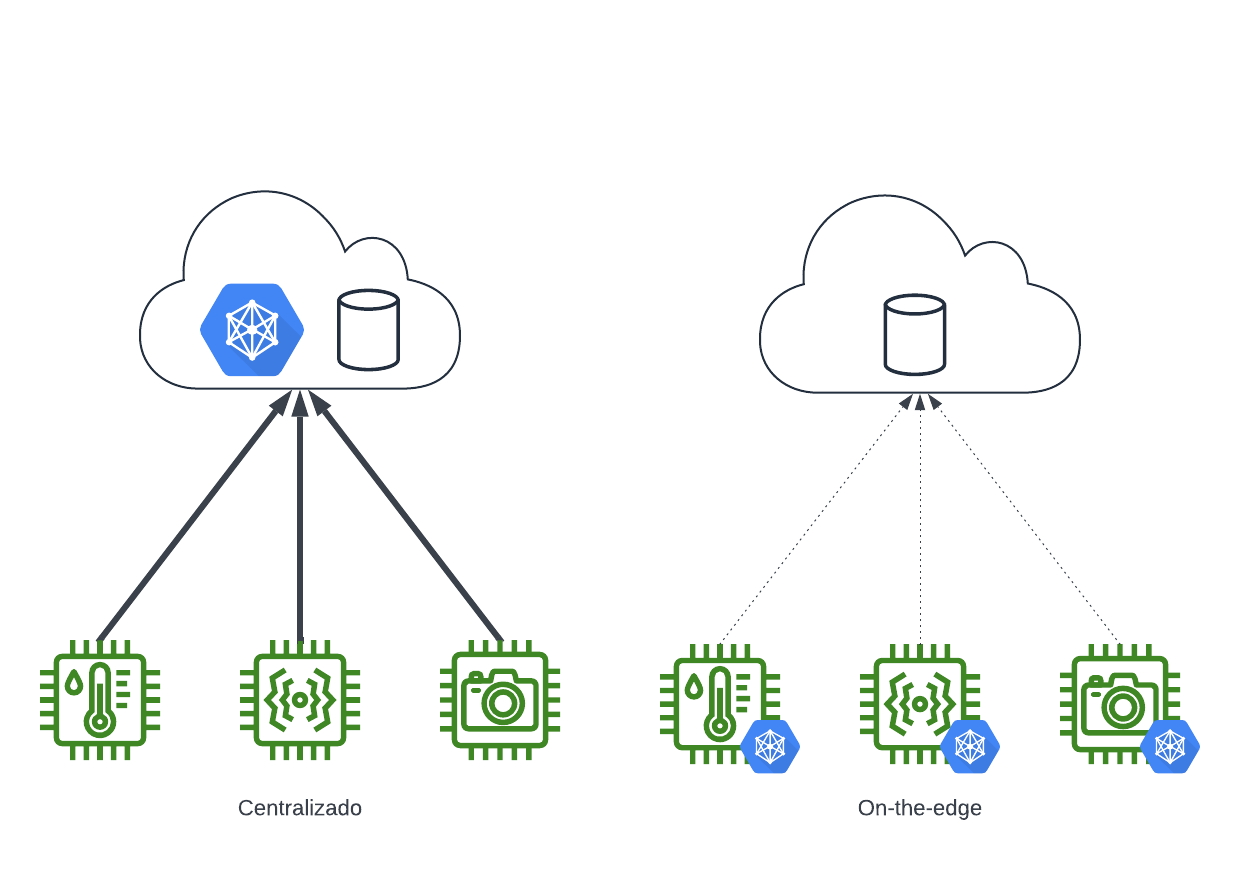
\includegraphics[height=.3\textheight]{./Figuras/EdgeVsCentralizedAI.png}
\caption{Diagrama de \textit{arquitecturas IoT}.}
\label{fig:EdgeVsCent}
\end{figure}

Entre las ventajas del enfoque descentralizado se encuentran:
\begin{itemize}
\item \textbf{Reducción de la latencia}: el procesamiento de datos en la nube puede ser lento, especialmente en entornos con una conexión de red de baja velocidad, algo muy utilizado en IoT ya que aumenta la duración de la batería que alimenta al nodo. Esto imposibilita su aplicación para aplicaciones en tiempo real, donde se debe obtener la salida del algoritmos en cuestión de menos de 1 segundo. El \textit{edge-computing} permite procesar los datos localmente, lo que reduce la latencia y mejora la respuesta del sistema.
\item \textbf{Mejora de la seguridad}: la transferencia de datos a la nube para procesamiento puede exponer información confidencial a riesgos de seguridad. El \textit{edge-computing} reduce el riesgo de acceso no autorizado a los datos, ya que se procesan localmente y solo se transmiten los resultados.
\item \textbf{Aumento de la eficiencia}: uno de los procesos que más energía consume IoT es la transmisión de datos, ya que generalmente ocurre a través de redes inalámbricas (WiFi, Bluetooth, LoRaWAN, etc). El \textit{edge-computing} reduce la cantidad de datos que es necesario transmitir, lo que genera ahorros de energía considerables. Esto es especialmente importante en dispositivos que deben funcionar durante años con baterías.
\item \textbf{Reducción de costos}: los servicios en la nube necesarios para ejecutar algoritmos de inteligencia artificial conllevan un costo de mantenimiento mensual que el cliente debe hacer frente cómo un gasto fijo operativo en su negocio. En ciertas aplicaciones, este gasto fijo se puede eliminar casi por completo utilizando un enfoque descentralizado. 
\end{itemize}

Las desventajas de utilizar una arquitectura descentralizada son:
\begin{itemize}
\item \textbf{Mayor costo de implementación}: la implementación de este tipo de sistemas puede requerir inversiones significativas en \textit{hardware} y \textit{software} especializados.
\item \textbf{Complejidad de mantenimiento}: el mantenimiento y actualización de estos sistemas distribuidos puede ser más complejo y costoso debido a la necesidad de gestionar múltiples dispositivos en simultaneo.
\item \textbf{Limitaciones de recursos y escalabilidad}: los dispositivos de \textit{edge-computing}, como los microcontroladores, suelen tener recursos limitados en términos de potencia de procesamiento, capacidad de almacenamiento y memoria. Esto puede dificultar la ejecución de aplicaciones de inteligencia artificial complejas y de alto rendimiento. Por esta razón, es crucial considerar desde las etapas iniciales del proyecto si esto puede llegar a limitar el crecimiento y la evolución futura del negocio.
\end{itemize}


\section{2. Identificación y análisis de los interesados}
\label{sec:interesados}

\begin{table}[ht]
%\caption{Identificación de los interesados}
%\label{tab:interesados}
\begin{tabularx}{\linewidth}{@{}|l|X|X|l|@{}}
\hline
\rowcolor[HTML]{C0C0C0} 
Rol           & Nombre y Apellido & Organización 	& Puesto 	\\ \hline
Cliente       & \clientename      &\empclientename	&        	\\ \hline
Responsable   & \authorname       & Very        	& Alumno 	\\ \hline
Colaboradores & \textcolor{red}{@todo Preguntar si Jose R?}                  &              	&        	\\ \hline
Orientador    & \supname	      & \pertesupname 	& Director Trabajo final \\ \hline
Usuario final & \clientename      &\empclientename	&        	\\ \hline
\end{tabularx}
\end{table}

\section{3. Propósito del proyecto}
\label{sec:proposito}

El propósito principal de este proyecto es sentar las bases para el desarrollo de aplicaciones de inteligencia artificial en sistemas embebidos, proporcionando a la empresa un repositorio que facilite las primeras etapas de nuevos proyectos de IA ``\textit{on-the-edge}". Esto permitirá comprender las capacidades y limitaciones de la IA en sistemas de recursos limitados, como los microprocesadores, y fomentará la eficiencia y viabilidad de futuros desarrollos en este campo.

\section{4. Alcance del proyecto}
\label{sec:alcance}

El alcance del proyecto se centra en el desarrollo de un repositorio \textit{template} para aplicaciones de inteligencia artificial en sistemas embebidos. El objetivo principal es proporcionar una base de herramientas que faciliten el desarrollo de aplicaciones de IA en plataformas de recursos limitados, como microcontroladores. También se incluirá un análisis de las posibilidades de esta tecnología para que \empclientename pueda tomar evaluar rápidamente si es viable su aplicación con un determinado cliente.

El proyecto incluirá los siguientes elementos:

\begin{enumerate}
\item Investigación del estado del arte en inteligencia artificial aplicada a sistemas embebidos.
\item Análisis y evaluación de librerías y \textit{frameworks} disponibles para el desarrollo de aplicaciones de IA en sistemas embebidos.
\item Selección de un microcontrolador adecuado para llevar a cabo análisis y pruebas de las aplicaciones de IA.
\item Creación de un repositorio en Github donde se desarrollará el repositorio \textit{template}.
\item Implementación de algoritmos de inteligencia artificial en el repositorio \textit{template}, incluyendo \textit{machine learning} clásico, \textit{deep learning} y, si es posible, visión por computadora.
\item Análisis de métricas para evaluar el rendimiento de los algoritmos implementados en términos de velocidad de ejecución, consumo de memoria y eficiencia energética. También se evaluará la precisión de los algoritmos comparándolo con el mismo modelo ejecutado en una computadora de uso general utilizando Python.
\item Conclusiones basadas en los resultados obtenidos en el análisis de métricas.
\end{enumerate}

El alcance del proyecto no incluye:
\begin{enumerate}
\item  El desarrollo completo de una aplicación de IA específica, sino que se centrará en proporcionar una base sólida y estructurada para futuros proyectos en este campo. 
\item No habrá recolección de datos para generar un \textit{dataset}. Para entrenar y evaluar los modelos, se utilizarán \textit{datasets} provistos por \empclientename o de uso público. 
\item La implementación de soluciones de \textit{edge computing} bajo el contexto específico de IoT, ni tampoco un análisis profundo respecto a la escalabilidad y flexibilidad de éstas arquitecturas. 
\item Desarrollar nuevas herramientas o tecnologías de inteligencia artificial en sistemas embebidos. El proyecto se centra en conocer y comprender el estado del arte actual en este campo, no en innovación dentro del mismo.
\item Los modelos de \textit{machine learning} no se entrenarán dentro del nodo.
\end{enumerate}


\section{5. Supuestos del proyecto}
\label{sec:supuestos}
Para el desarrollo del presente proyecto se supone que: 
\begin{itemize}
	\item Los microcontroladores disponibles comercialmente son capaces de ejecutar los algoritmos de inteligencia artificial implementados en el repositorio \textit{template}.
	\item Existen librerías y \textit{frameworks} disponibles que sean adecuados para el desarrollo de aplicaciones de IA en sistemas embebidos.
	\item Se tiene una disponibilidad horaria de al menos 600 horas laborales del responsable para realizar el trabajo. 
	\item \empclientename proporcionará el tiempo y recursos necesarios para poder progresar en la implementación de los algoritmos.
	\item Los conocimientos adquiridos en el posgrado son suficientes para aplicar las técnicas de IA deseadas.
\end{itemize}


\section{6. Requerimientos}
\label{sec:requerimientos}

Aclaración: en este proyecto se implementarán múltiples modelos de \textit{machine learning} para evaluar su performance. Por lo tanto, los requerimientos funcionales son genéricos y aplican a todos los modelos a implementar siempre que sea posible. A partir de los requerimientos planteados, se podrá analizar las limitaciones de cada algoritmo y compararlos.

\begin{enumerate}
	\item Requerimientos funcionales de los modelos de \textit{machine learning}: 
		\begin{enumerate}
			\item El código del modelo debe estar encapsulado dentro de un módulo y debe contar con una API para acceder a las principales funciones del mismo.
			\item El modelo debe tener la capacidad de actualizar sus pesos sin la necesidad de una actualización completa de \textit{firmware}, siempre y cuando no se modifique la arquitectura del algoritmo.
			\item El módulo de \textit{machine learning} contará con metadata que permitirá identificar el tipo de algoritmo, versión del modelo y versión de los pesos.
			\item El módulo de \textit{machine learning} debe permitir la extracción de muestras de validación que incluirán: datos de entrada, datos y métricas de salida y metadata del modelo. Esto facilitará la validación de los algoritmos cuando el sistema se encuentre en producción.
			\item El módulo debe ser capaz de medir el tiempo de ejecución del algoritmo y generar métricas estadísticas del uso del CPU y RAM.
		\end{enumerate}
	\item Requerimientos de documentación
		\begin{enumerate}
			\item La documentación debe mantenerse dentro del mismo repositorio de Github.
			\item La documentación debe indicar los pasos para instalar el ambiente de desarrollo, incluyendo la instalación de librerías y módulos necesarios.
			\item La documentación debe indicar los pasos para ejecutar cada una de las pruebas que se llevaron a cabo durante el proyecto.
			\item La documentación debe registrar la investigación realizada en el proyecto, identificando claramente las limitaciones de las tecnologías utilizadas.
			\item La documentación debe indicar los requerimientos mínimos recomendables de \textit{hardware} para ejecutar este tipo de aplicaciones.
		\end{enumerate}
	\item Requerimientos funcionales de la interfaz de comunicación
		\begin{enumerate}
		\item El sistema debe contar con un módulo de comunicación que permitirá enviar y recibir datos con una PC conectada por USB.
		\item El protocolo de comunicación debe validar la integridad de los datos.
		\item La PC debe ser capaz de comunicarse con el nodo para:
			\begin{enumerate}
				\item Obtener información del nodo: versión del código, metadata del modelo de \textit{machine learning}
				\item Actualizar los pesos del algoritmo de \textit{machine learning}
			\end{enumerate}
		\end{enumerate}
	\item Requerimiento de testing
		\begin{enumerate}
			\item Los modelos de \textit{machine learning} ejecutados en el nodo serán comparados contra las métricas obtenido de ejecutar los mismos modelos en una PC, utilizando Python.
			\item La ejecución de las pruebas debe ser automática mediante un \textit{script}.
		\end{enumerate}
\end{enumerate}

\section{7. Historias de usuarios (\textit{Product backlog})}
\label{sec:backlog}

\underline{Roles:} 
\begin{itemize}
\item Evaluador: es quien va a evaluar si utilizar algoritmos de \textit{machine learning} en los nodos es una alternativa viable para el proyecto. Esta persona cuenta con conocimientos técnicos, aunque no necesariamente sea especialista en desarrollos de inteligencia artificial o \textit{firmware}.
\item Desarrollador: es la persona que, una vez evaluada la viabilidad de la tecnología para un proyecto, utilizará el repositorio como base de desarrollo para un modelo de inteligencia artificial específico. Esta persona cuenta con conocimientos técnicos en programación, inteligencia artificial y sistemas embebidos.
\end{itemize}


\underline{\textit{Story points}:} 
\begin{table}[h]
\centering
\renewcommand{\tabularxcolumn}{m} % we want center vertical alignment

\begin{tabularx}{\textwidth}{|c|>{\raggedright}X|}
\hline
\textbf{Puntaje \#} & \textbf{Descripción:} \tabularnewline
\hline
1 & Estos son detalles menores o implementaciones simples que se estiman se pueden resolver en horas o en un solo día.\tabularnewline
\hline
3 & Se estima que la ejecución de este tipo de tarea puede tomar hasta un tercio del sprint. \tabularnewline
\hline
5 & Se espera que trabajar en este tipo de historia utilice aproximadamente dos tercios de la capacidad del sprint. \tabularnewline
\hline
8 & Estas son las historias más complejas o difíciles de implementar y se estima que pueden tomar todo el sprint. \tabularnewline
\hline
\end{tabularx}
\end{table}


\underline{Historias de usuario:} 
\begin{itemize}
\item Como evaluador, quiero tener fácil acceso al tiempo de ejecución de los algoritmos. Esto me permitirá evaluar si el consumo es demasiado elevado para, por ejemplo, un sistema que funciona con baterías (Puntos: 3).
\item Como evaluador, quiero ver métricas de la ejecución de los algoritmos que sean independientes del microprocesador utilizado, para así poder extrapolar las conclusiones a otras plataformas (Puntos: 8).
\item Como evaluador, quiero ver fácilmente qué tipos de algoritmos de inteligencia artificial se pueden ejecutar en sistemas embebidos de recursos limitados  (Puntos: 1).
\item Como evaluador, quiero conocer las limitaciones de este tipo de tecnologías, para descartar rápidamente en el caso de que no sea compatible con el proyecto que se quiere desarrollar  (Puntos: 5).
\item Como desarrollador, quiero tener instrucciones claras para configurar el entorno de desarrollo y así comenzar el desarrollo llo más pronto posible  (Puntos: 3).
\item Como desarrollador, quiero entender las limitaciones de los algoritmos de \textit{machine learning} que se pueden ejecutar en estos sistemas, para desarrollar un modelo acorde (Puntos: 3).
\item Como desarrollador, quiero poder actualizar los pesos del modelo fácilmente para poder iterar de forma eficiente  (Puntos: 8).
\item Como desarrollador, quiero poder tener acceso a las variables internas del modelo siendo ejecutado en el microprocesador, de forma tal de poder validar que el algoritmo se está ejecutando según lo esperado (Puntos: 5).
\end{itemize}

\section{8. Entregables principales del proyecto}
\label{sec:entregables}

Los entregables del proyecto son:
\begin{itemize}
	\item Módulos de \textit{machine learning} con distintos modelos implementados.
	\item Ejemplos de uso de los algoritmos.
	\item Análisis del estado del arte y performance de los modelos.
	\item Documentación de instalación del entorno de desarrollo.
\end{itemize}

\section{9. Desglose del trabajo en tareas}
\label{sec:wbs}

\begin{enumerate}
\item Investigación y planificación
	\begin{enumerate}
	\item Investigación del estado del arte (32 hs)
	\item Definición de modelos de \textit{machine learning} a implementar (24 hs)
	\item Selección de los datasets a utilizar para las pruebas de cada modelo (24 hs)
	\item Selección de la plataforma (microcontrolador) donde se llevarán a cabo las pruebas (24 hs)
	\item Diseñar arquitectura de firmware del nodo (16 hs)
	\end{enumerate}
\item Desarrollo de estructura base
	\begin{enumerate}
	\item Configurar entorno de desarrollo (24 hs)
	\item Implementar arquitectura de firmware (40 hs)
	\item Implementar protocolo de comunicación (20 hs)
	\item Desarrollar script de interacción nodo-PC (24 hs)
	\item Implementar flujo del programa: adquisición de datos -> procesamiento -> predicción (40 hs)
	\end{enumerate}
\item Desarrollo de algoritmos de inteligencia artificial
	\begin{enumerate}
	\item Diseñar módulo de IA y APIs (40 hs)
	\item Entrenar modelos en Python (40 hs)
	\item Desplegar modelos de IA en nodo (40 hs)
	\item Generar muestras de validación y envíar a la PC (24 hs)
	\item Testing del funcionamiento de los algoritmos (20 hs) 
	\item Agregar mecanismos de evaluación de performance dentro del código (20 hs)
	\item Adaptar código para permitir la actualización de pesos del modelo (32 hs) 
	\end{enumerate}
\item Documentación
	\begin{enumerate}
	\item Documentar análisis realizado (20 hs)
	\item Documentar conclusiones de los modelos implementados y aspectos a tomar en cuenta respecto a la plataforma utilizada. (30 hs)
	\item Redacción del informe de avance (16 hs).
	\item Redacción de la memoria del proyecto (40 hs).
	\item Preparación de la presentación pública (10 hs).
	\end{enumerate}
\end{enumerate}

Cantidad total de horas: (600 h)

\section{10. Diagrama de Activity On Node}
\label{sec:AoN}

\begin{consigna}{red}
Armar el AoN a partir del WBS definido en la etapa anterior. 

%La figura \ref{fig:AoN} fue elaborada con el paquete latex tikz y pueden consultar la siguiente referencia \textit{online}:

%\url{https://www.overleaf.com/learn/latex/LaTeX_Graphics_using_TikZ:_A_Tutorial_for_Beginners_(Part_3)\%E2\%80\%94Creating_Flowcharts}

\end{consigna}

\begin{figure}[htpb]
\centering 
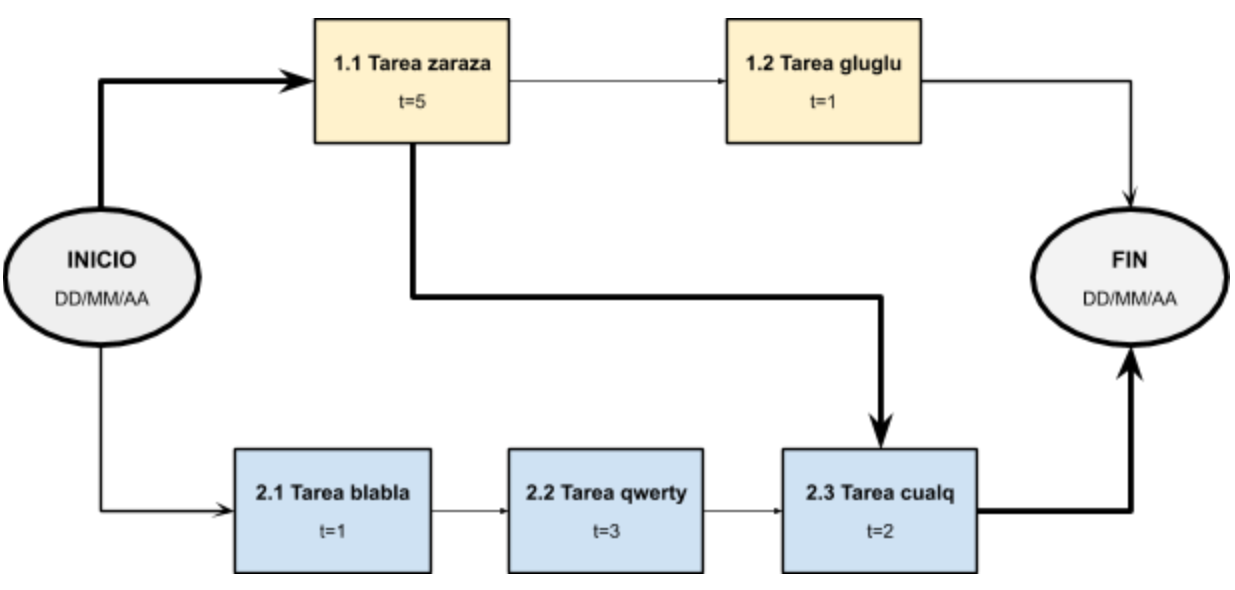
\includegraphics[width=.8\textwidth]{./Figuras/AoN.png}
\caption{Diagrama de \textit{Activity on Node}.}
\label{fig:AoN}
\end{figure}

Indicar claramente en qué unidades están expresados los tiempos.
De ser necesario indicar los caminos semicríticos y analizar sus tiempos mediante un cuadro.
Es recomendable usar colores y un cuadro indicativo describiendo qué representa cada color, como se muestra en el siguiente ejemplo:



\section{11. Diagrama de Gantt}
\label{sec:gantt}

\begin{consigna}{red}

Existen muchos programas y recursos \textit{online} para hacer diagramas de Gantt, entre los cuales destacamos:

\begin{itemize}
\item Planner
\item GanttProject
\item Trello + \textit{plugins}. En el siguiente link hay un tutorial oficial: \\ \url{https://blog.trello.com/es/diagrama-de-gantt-de-un-proyecto}
\item Creately, herramienta online colaborativa. \\\url{https://creately.com/diagram/example/ieb3p3ml/LaTeX}
\item Se puede hacer en latex con el paquete \textit{pgfgantt}\\ \url{http://ctan.dcc.uchile.cl/graphics/pgf/contrib/pgfgantt/pgfgantt.pdf}
\end{itemize}

Pegar acá una captura de pantalla del diagrama de Gantt, cuidando que la letra sea suficientemente grande como para ser legible. 
Si el diagrama queda demasiado ancho, se puede pegar primero la ``tabla'' del Gantt y luego pegar la parte del diagrama de barras del diagrama de Gantt.

Configurar el software para que en la parte de la tabla muestre los códigos del EDT (WBS).\\
Configurar el software para que al lado de cada barra muestre el nombre de cada tarea.\\
Revisar que la fecha de finalización coincida con lo indicado en el Acta Constitutiva.

En la figura \ref{fig:gantt}, se muestra un ejemplo de diagrama de Gantt realizado con el paquete de \textit{pgfgantt}. En la plantilla pueden ver el código que lo genera y usarlo de base para construir el propio.

\begin{figure}[htbp]
\begin{center}
\begin{ganttchart}{1}{12}
  \gantttitle{2020}{12} \\
  \gantttitlelist{1,...,12}{1} \\
  \ganttgroup{Group 1}{1}{7} \\
  \ganttbar{Task 1}{1}{2} \\
  \ganttlinkedbar{Task 2}{3}{7} \ganttnewline
  \ganttmilestone{Milestone o hito}{7} \ganttnewline
  \ganttbar{Final Task}{8}{12}
  \ganttlink{elem2}{elem3}
  \ganttlink{elem3}{elem4}
\end{ganttchart}
\end{center}
\caption{Diagrama de Gantt de ejemplo}
\label{fig:gantt}
\end{figure}


\begin{landscape}
\begin{figure}[htpb]
\centering 
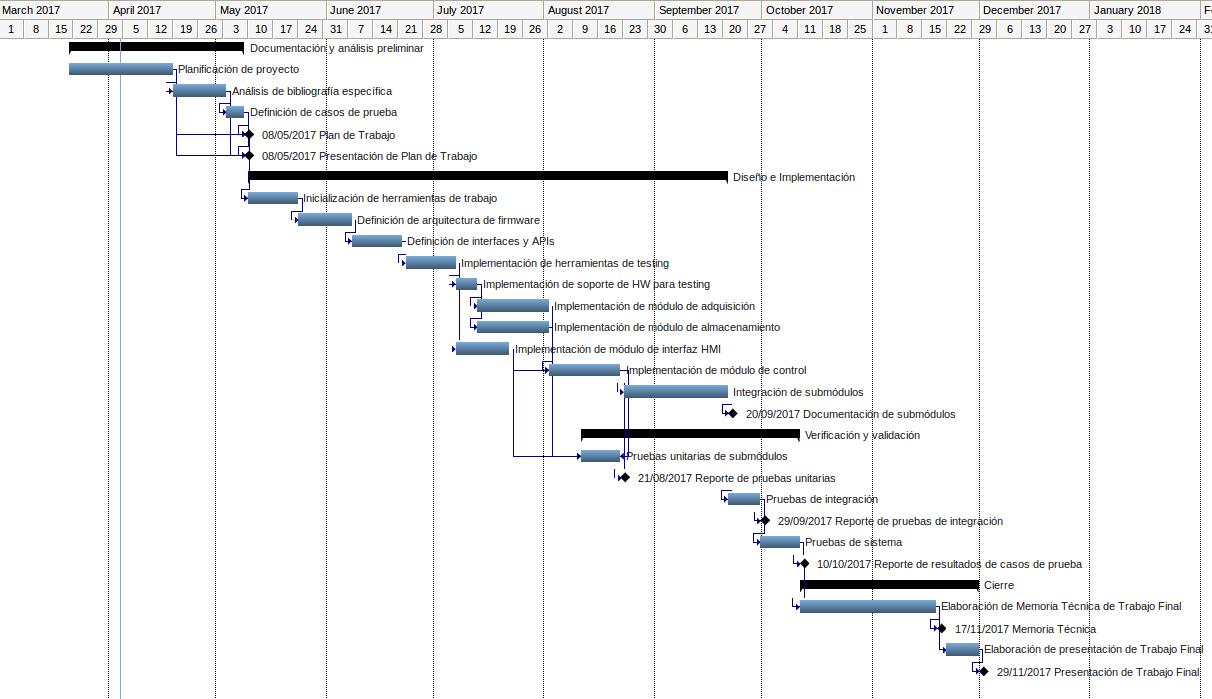
\includegraphics[height=.85\textheight]{./Figuras/Gantt-2.png}
\caption{Ejemplo de diagrama de Gantt rotado}
\label{fig:diagGantt}
\end{figure}

\end{landscape}

\end{consigna}


\section{12. Presupuesto detallado del proyecto}
\label{sec:presupuesto}

\begin{consigna}{red}
Si el proyecto es complejo entonces separarlo en partes:
\begin{itemize}
	\item Un total global, indicando el subtotal acumulado por cada una de las áreas.
	\item El desglose detallado del subtotal de cada una de las áreas.
\end{itemize}

IMPORTANTE: No olvidarse de considerar los COSTOS INDIRECTOS.

\end{consigna}

\begin{table}[htpb]
\centering
\begin{tabularx}{\linewidth}{@{}|X|c|r|r|@{}}
\hline
\rowcolor[HTML]{C0C0C0} 
\multicolumn{4}{|c|}{\cellcolor[HTML]{C0C0C0}COSTOS DIRECTOS} \\ \hline
\rowcolor[HTML]{C0C0C0} 
Descripción &
  \multicolumn{1}{c|}{\cellcolor[HTML]{C0C0C0}Cantidad} &
  \multicolumn{1}{c|}{\cellcolor[HTML]{C0C0C0}Valor unitario} &
  \multicolumn{1}{c|}{\cellcolor[HTML]{C0C0C0}Valor total} \\ \hline
 &
  \multicolumn{1}{c|}{} &
  \multicolumn{1}{c|}{} &
  \multicolumn{1}{c|}{} \\ \hline
 &
  \multicolumn{1}{c|}{} &
  \multicolumn{1}{c|}{} &
  \multicolumn{1}{c|}{} \\ \hline
\multicolumn{1}{|l|}{} &
   &
   &
   \\ \hline
\multicolumn{1}{|l|}{} &
   &
   &
   \\ \hline
\multicolumn{3}{|c|}{SUBTOTAL} &
  \multicolumn{1}{c|}{} \\ \hline
\rowcolor[HTML]{C0C0C0} 
\multicolumn{4}{|c|}{\cellcolor[HTML]{C0C0C0}COSTOS INDIRECTOS} \\ \hline
\rowcolor[HTML]{C0C0C0} 
Descripción &
  \multicolumn{1}{c|}{\cellcolor[HTML]{C0C0C0}Cantidad} &
  \multicolumn{1}{c|}{\cellcolor[HTML]{C0C0C0}Valor unitario} &
  \multicolumn{1}{c|}{\cellcolor[HTML]{C0C0C0}Valor total} \\ \hline
\multicolumn{1}{|l|}{} &
   &
   &
   \\ \hline
\multicolumn{1}{|l|}{} &
   &
   &
   \\ \hline
\multicolumn{1}{|l|}{} &
   &
   &
   \\ \hline
\multicolumn{3}{|c|}{SUBTOTAL} &
  \multicolumn{1}{c|}{} \\ \hline
\rowcolor[HTML]{C0C0C0}
\multicolumn{3}{|c|}{TOTAL} &
   \\ \hline
\end{tabularx}%
\end{table}


\section{13. Gestión de riesgos}
\label{sec:riesgos}

\begin{consigna}{red}
a) Identificación de los riesgos (al menos cinco) y estimación de sus consecuencias:
 
Riesgo 1: detallar el riesgo (riesgo es algo que si ocurre altera los planes previstos de forma negativa)
\begin{itemize}
	\item Severidad (S): mientras más severo, más alto es el número (usar números del 1 al 10).\\
	Justificar el motivo por el cual se asigna determinado número de severidad (S).
	\item Probabilidad de ocurrencia (O): mientras más probable, más alto es el número (usar del 1 al 10).\\
	Justificar el motivo por el cual se asigna determinado número de (O). 
\end{itemize}   

Riesgo 2:
\begin{itemize}
	\item Severidad (S): 
	\item Ocurrencia (O):
\end{itemize}

Riesgo 3:
\begin{itemize}
	\item Severidad (S): 
	\item Ocurrencia (O):
\end{itemize}


b) Tabla de gestión de riesgos:      (El RPN se calcula como RPN=SxO)

\begin{table}[htpb]
\centering
\begin{tabularx}{\linewidth}{@{}|X|c|c|c|c|c|c|@{}}
\hline
\rowcolor[HTML]{C0C0C0} 
Riesgo & S & O & RPN & S* & O* & RPN* \\ \hline
       &   &   &     &    &    &      \\ \hline
       &   &   &     &    &    &      \\ \hline
       &   &   &     &    &    &      \\ \hline
       &   &   &     &    &    &      \\ \hline
       &   &   &     &    &    &      \\ \hline
\end{tabularx}%
\end{table}

Criterio adoptado: 
Se tomarán medidas de mitigación en los riesgos cuyos números de RPN sean mayores a...

Nota: los valores marcados con (*) en la tabla corresponden luego de haber aplicado la mitigación.

c) Plan de mitigación de los riesgos que originalmente excedían el RPN máximo establecido:
 
Riesgo 1: plan de mitigación (si por el RPN fuera necesario elaborar un plan de mitigación).
  Nueva asignación de S y O, con su respectiva justificación:
  - Severidad (S): mientras más severo, más alto es el número (usar números del 1 al 10).
          Justificar el motivo por el cual se asigna determinado número de severidad (S).
  - Probabilidad de ocurrencia (O): mientras más probable, más alto es el número (usar del 1 al 10).
          Justificar el motivo por el cual se asigna determinado número de (O).

Riesgo 2: plan de mitigación (si por el RPN fuera necesario elaborar un plan de mitigación).
 
Riesgo 3: plan de mitigación (si por el RPN fuera necesario elaborar un plan de mitigación).

\end{consigna}


\section{14. Gestión de la calidad}
\label{sec:calidad}

\begin{consigna}{red}
Elija al menos diez requerientos que a su criterio sean los más importantes/críticos/que aportan más valor y para cada uno de ellos indique las acciones de verificación y validación que permitan asegurar su cumplimiento.

\begin{itemize} 
\item Req \#1: copiar acá el requerimiento.

\begin{itemize}
	\item Verificación para confirmar si se cumplió con lo requerido antes de mostrar el sistema al cliente. Detallar 
	\item Validación con el cliente para confirmar que está de acuerdo en que se cumplió con lo requerido. Detallar  
\end{itemize}

\end{itemize}

Tener en cuenta que en este contexto se pueden mencionar simulaciones, cálculos, revisión de hojas de datos, consulta con expertos, mediciones, etc.  Las acciones de verificación suelen considerar al entregable como ``caja blanca'', es decir se conoce en profundidad su funcionamiento interno.  En cambio, las acciones de validación suelen considerar al entregable como ``caja negra'', es decir, que no se conocen los detalles de su funcionamiento interno.

\end{consigna}

\section{15. Procesos de cierre}    
\label{sec:cierre}

\begin{consigna}{red}
Establecer las pautas de trabajo para realizar una reunión final de evaluación del proyecto, tal que contemple las siguientes actividades:

\begin{itemize}
	\item Pautas de trabajo que se seguirán para analizar si se respetó el Plan de Proyecto original:
	 - Indicar quién se ocupará de hacer esto y cuál será el procedimiento a aplicar. 
	\item Identificación de las técnicas y procedimientos útiles e inútiles que se emplearon, y los problemas que surgieron y cómo se solucionaron:
	 - Indicar quién se ocupará de hacer esto y cuál será el procedimiento para dejar registro.
	\item Indicar quién organizará el acto de agradecimiento a todos los interesados, y en especial al equipo de trabajo y colaboradores:
	  - Indicar esto y quién financiará los gastos correspondientes.
\end{itemize}

\end{consigna}


\end{document}
